\documentclass[11pt]{article}

\usepackage[margin=1in]{geometry}
\usepackage{amsmath,amssymb}
\usepackage{booktabs}
\usepackage{graphicx}
\usepackage{float}
\usepackage{xcolor}
\usepackage{hyperref}
\graphicspath{{figs/}{../../}}

\newcommand{\plain}[1]{\medskip\noindent\fbox{\parbox{0.95\linewidth}{\textbf{Verdict.} #1}}\medskip}
\newcommand{\pending}[1]{\medskip\noindent\fcolorbox{gray}{gray!12}{\parbox{0.95\linewidth}{\textbf{TO DO (experiment not finished).} #1}}\medskip}

\title{What Makes Neural Networks Easy to Fool?\\
A Controlled Tour of the Candidate Root Causes}
\author{Ali Kayyam\\\texttt{akayyam@brainchip.com}}
\date{DRAFT}

\begin{document}
\sloppy
\maketitle

\begin{abstract}
Networks are now far more robust to small, deliberate changes than they were a few years ago, yet there is still no agreed answer to the basic question: \emph{what is the core issue?} Many explanations have been proposed: networks add up many tiny effects, they rely on predictive but fragile features, they prefer texture to shape, their models are not sparse, they ignore directions the data never explores, they have too little data, or training simply finds the wrong solution. They are rarely compared on equal terms.
This paper is an illustrative study for junior researchers and curious readers. We test each explanation on its own, in a small problem where the truth is known, with one yardstick throughout: the smallest change that flips the model's answer, and how it compares with the best that any model could do. We organise the findings around one split. Some vulnerability is \emph{inevitable}: given the data and the allowed change, no model can be both accurate and robust. The rest is \emph{avoidable}: a better model exists, but the objective, the optimiser, the architecture or the data do not find it.
In our toy worlds, the dominant effect is the inevitable one, namely evidence spread over many inputs under a per-input budget. It also accounts for shape versus texture: for the best possible rule only how widely a cue is spread matters, not its frequency. On top of it we find avoidable effects that are real but smaller: ignoring irrelevant inputs (up to $2\times$), a convolutional network that reads fine textures badly, optimiser bias towards the wrong kind of solution, and sensitivity off the data manifold, which disappears with weight decay. A network trained only on adversarial changes still learns the true classes, so the changes are made of real features. More data does not change vulnerability under standard training, in the toy world or on real data. Adversarial training reaches the inevitable ceiling in the toy world, so the avoidable gap there is a gap in the objective; on real data it raises flip sizes by $1.5$--$6\times$ at a cost of up to a few points of clean accuracy, and its robust accuracy then depends strongly on the amount of data.
Checks on MNIST, Fashion-MNIST and CIFAR-10 confirm several of these effects (irrelevant inputs nearly halve the flip size, the $\ell_\infty$ max-margin solution beats the $\ell_2$ one by about $50\%$, adversarial changes carry learnable features) and qualify others: sensitivity off the main principal components appears on CIFAR-10 but not MNIST, and we find no special fragility to high frequencies. Wider and deeper networks (a $1024$-unit MLP, ResNet-18) show the same picture. It is an aid to intuition and a map of causes, not a claim about large networks in general.
\end{abstract}

\section{The puzzle and a way to organise the answer}

A faint pattern of noise, invisible to a person, makes an accurate image classifier change its answer. Adversarial training and other defences now make models much more robust, but we still lack a clear account of \emph{why} ordinary models are fragile in the first place. The literature offers many candidate causes~\cite{szegedy2014,goodfellow2015,tsipras2019,ilyas2019,geirhos2019}; each is usually shown on its own, on a different dataset, with a different measure.

We do two things. First, we compare candidate causes in the same small, fully controlled worlds with the same measure. Second, we sort what we find using one distinction.

\begin{itemize}
\item \textbf{Inevitable (data-limited).} Given the data and the allowed change $\epsilon$, no classifier can be both accurate and robust. The classes overlap within $\epsilon$, or the evidence is spread so thinly that robustness costs accuracy.
\item \textbf{Avoidable (learning-limited).} A classifier that is accurate \emph{and} robust exists, but the training objective, the optimiser, the architecture or the amount of data does not find it.
\end{itemize}

Figure~\ref{fig:illa} shows the two cases in a picture. Every hypothesis below is a claim about which part it explains. A cause that is \emph{necessary} must appear whenever vulnerability does; a cause that is \emph{sufficient} produces vulnerability by itself; a cause may also only \emph{contribute}. Our scorecard (Section~\ref{sec:score}) records which, with a plain statement of how strong the evidence is.

\begin{figure}[H]
\centering
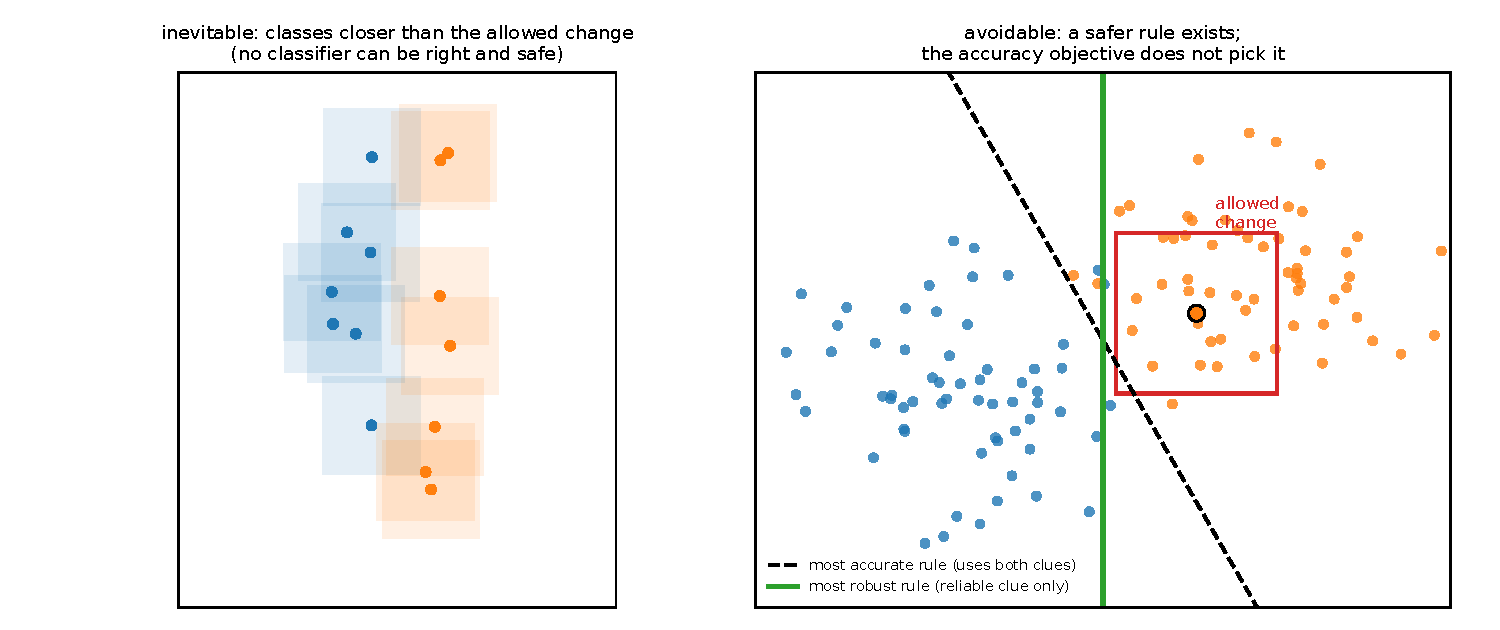
\includegraphics[width=0.92\textwidth]{ill_a_split.pdf}
\caption{Two kinds of vulnerability. Left: when the allowed change (squares around each point) is larger than the gap between the classes, no classifier can be both right and safe: inevitable. Right: two clues, one reliable and one weak. The most accurate rule (dashed) uses both and tilts; the most robust rule (green) uses the reliable clue only. A change within the red square flips the accurate rule's answer for the marked point but not the robust rule's: avoidable, but only by changing what training asks for.}
\label{fig:illa}
\end{figure}

\paragraph{The yardstick.} For every model and every correctly classified test point we compute the \emph{flip size}: the smallest change that flips the answer. We measure it two ways: the largest change to any single input (per-input, $\ell_\infty$) and the length of the whole change (total, $\ell_2$). Their ratio tells how widely the model spreads its attention. Where the data are generated by us, we also compute the same quantity exactly for the best possible rule.

\paragraph{How to read the paper.} Each subsection asks one question, runs one small experiment, and ends with a boxed verdict. Settings are in Appendix~\ref{app:settings}; unless stated, numbers are means over 10 runs.

\section{The toy world}
\label{sec:world}

Every example is six numbers and a label $0$ or $1$ with equal chance. The first number is a \emph{reliable clue} (its class averages are $1.0$ apart; looking at it alone gives $95\%$ accuracy). The other five are \emph{weak clues} (class averages $0.4$ apart; each alone gives $79\%$). The noise is bell-shaped and the values are not clipped, so the best possible rule is a weighted sum of the six numbers, answered by its sign. It reaches $99.3\%$. Five weak clues together reach $96.3\%$, better than the reliable clue alone. A small network (one hidden layer of 8 units) trained on this task reaches the same accuracy.

For a weighted sum with weights $w_i$ and total $\sum_i w_i x_i$, an attacker who may change every input by at most $\epsilon$ moves the total by $\epsilon\sum_i |w_i|=\epsilon\|w\|_1$. The answer flips when this exceeds the answer's confidence, so
\[
\text{per-input flip size}=\frac{\text{confidence}}{\|w\|_1},\qquad
\text{total flip size}=\frac{\text{confidence}}{\|w\|_2}.
\]
This one formula organises most of what follows. It is exact for the best rule; for trained networks we find the flip size by search.

\section{The tour}

\subsection{H1: evidence added up over many inputs}
\label{sec:h1}

\textbf{Claim} (Goodfellow et al.~\cite{goodfellow2015}; see also Simon-Gabriel et al.~\cite{simongabriel2019}): a small change to every input, all in the unhelpful direction, adds up. \textbf{Experiment:} keep the total evidence fixed and split it equally over $k=1,2,\ldots,64$ inputs, so accuracy stays at $95\%$ (Figure~\ref{fig:h1}).

\begin{figure}[H]
\centering
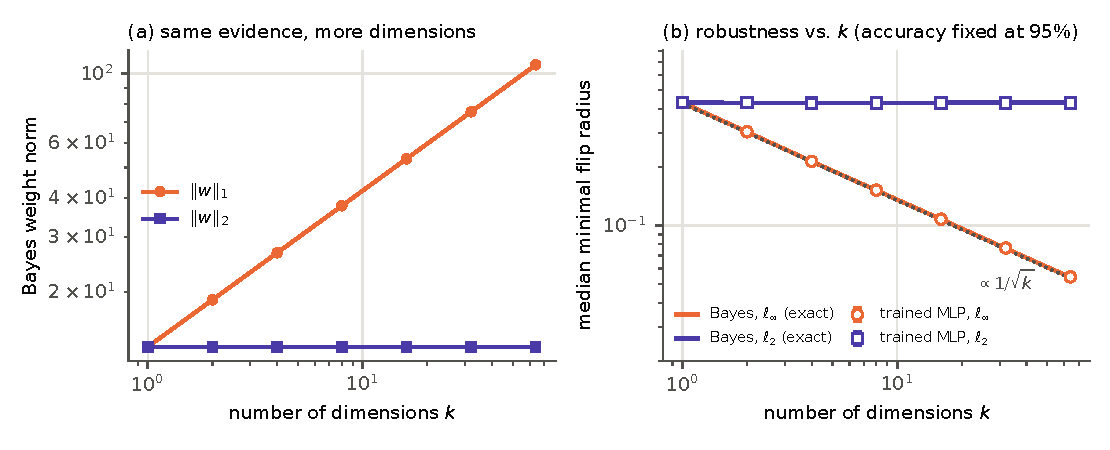
\includegraphics[width=0.95\textwidth]{fig_rc_dimensions.pdf}
\caption{Same evidence spread over $k$ inputs. Per-input flip size (steep lines) falls as $1/\sqrt k$; total flip size (flat lines) does not move. Exact best rule (lines) and trained networks (markers) coincide.}
\label{fig:h1}
\end{figure}

Figure~\ref{fig:geom} shows why in two dimensions: the square of allowed per-input changes reaches a diagonal boundary with a smaller side than it needs for an axis-aligned one, although the straight-line distance (the circle) is the same.

\begin{figure}[H]
\centering
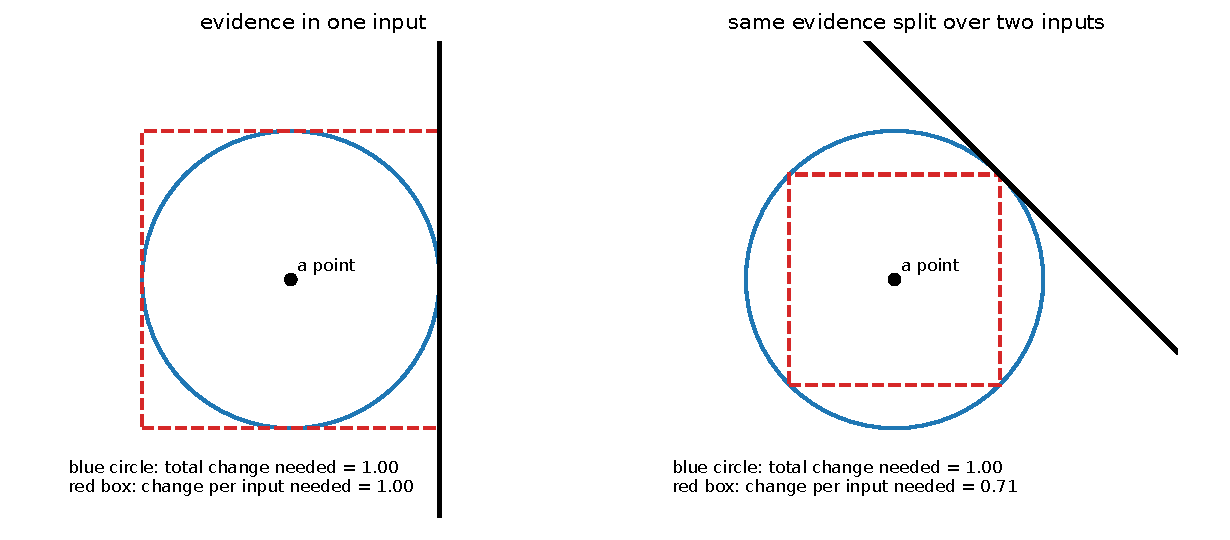
\includegraphics[width=0.8\textwidth]{fig_il_geometry.pdf}
\caption{Two inputs, one point. Blue circle: total change needed to reach the decision boundary (black). Red dashed square: per-input change needed. Splitting the evidence over two inputs leaves the circle unchanged and shrinks the square.}
\label{fig:geom}
\end{figure}

The per-input flip size falls from $0.43$ at $k=1$ to $0.054$ at $k=64$ (a factor of eight), with the same accuracy and the same total flip size ($0.43$). The trained network lies on the exact curve.

\plain{Necessary and sufficient, in this world, for fragility to small per-input changes. It is \emph{inevitable}: the best rule has it too. It disappears if the attacker is limited by total size ($\ell_2$) instead, so it is a statement about the pairing of the data with the allowed change.}

\subsection{H2: small clues, not unreliable ones}
\label{sec:h2}

\textbf{Claim} (Ilyas et al.~\cite{ilyas2019}): networks rely on features that are predictive but fragile. \textbf{Experiment:} one clue; vary its size (gap between class averages) and its reliability independently (Figure~\ref{fig:h2}).

\begin{figure}[H]
\centering
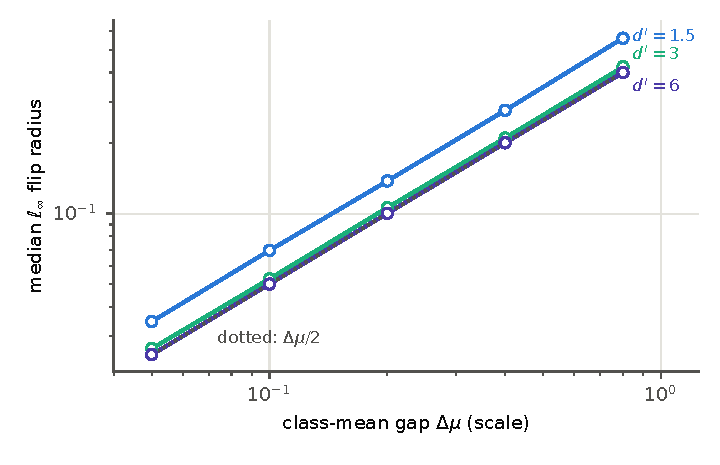
\includegraphics[width=0.55\textwidth]{fig_rc_scale.pdf}
\caption{Flip size of a single clue against its size, at three reliabilities. The lines nearly coincide: size matters, reliability hardly does.}
\label{fig:h2}
\end{figure}

Flip size is proportional to the clue's size. Raising reliability from $77\%$ to $99.9\%$ changes it by only about $1.4\times$, and in the wrong direction for the usual intuition: a more reliable clue is slightly \emph{easier} to flip. A clue that is $99.9\%$ reliable but tiny (gap $0.05$) flips at $0.025$.

\plain{``Non-robust'' means small relative to the allowed change, not unreliable. Inevitable (a property of the data). Still to do: the transfer test (do changes crafted against a small-scale-feature model fool a large-scale-feature model?).}

\paragraph{Transfer test: are adversarial changes made of real features?} Ilyas et al.~\cite{ilyas2019} showed that a network trained only on adversarially changed images, with labels given by the \emph{target} of the change, can still classify clean images. We repeat this in miniature. For each training point we craft a targeted change of size $\epsilon$ towards a randomly chosen target label and keep the changed input with that target label. The labels are random with respect to the true class, so a fresh network can do well on clean data only if the changes themselves carry features (Figure~\ref{fig:h2b}).

\begin{figure}[H]
\centering
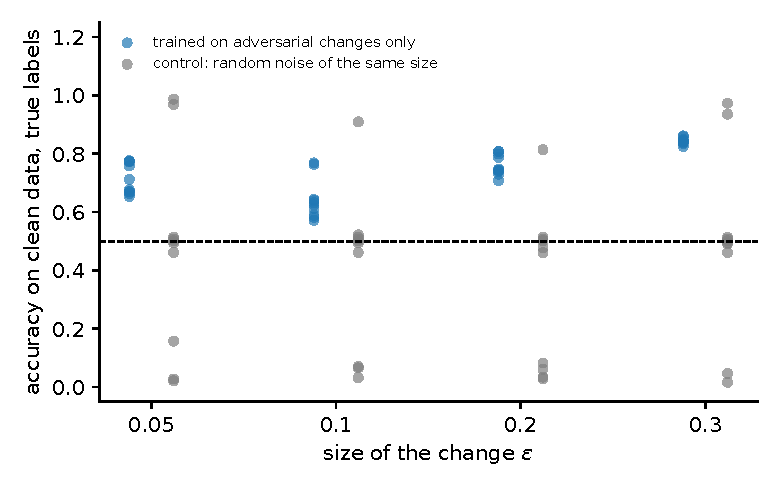
\includegraphics[width=0.55\textwidth]{h2b_transfer.pdf}
\caption{Accuracy on clean data (true labels) of a fresh network trained only on adversarially changed inputs with random target labels (blue, 10 runs), against a control trained on random-sign noise of the same size (gray).}
\label{fig:h2b}
\end{figure}

The fresh network is above chance in every one of the 10 runs at every $\epsilon$ (mean $0.71$, $0.64$, $0.76$, $0.84$ for $\epsilon=0.05,0.1,0.2,0.3$). The control scatters between $0.02$ and $0.99$: an almost untrained network lines up with the reliable clue by chance, positively or negatively, and shows no consistent signal.

\plain{In this world an adversarial change is built from the data's own predictive directions. This supports the ``features, not bugs'' reading in its simplest form. It is unsurprising for a weighted sum, which is the point: very little needs to be assumed.}

\subsection{H4: sparsity}
\label{sec:h4}

Sparsity can mean three different things. We test each.

\paragraph{(a) Sparse versus dense signal.} Put the same total evidence in $s$ of 64 inputs; the other $64-s$ inputs are pure noise (Figure~\ref{fig:h4a}).

\begin{figure}[H]
\centering
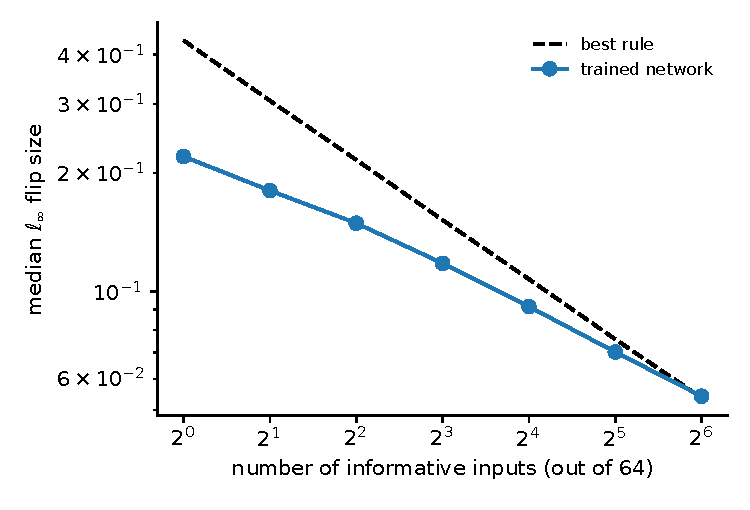
\includegraphics[width=0.5\textwidth]{h4a_sparse.pdf}
\caption{Median per-input flip size against the number of informative inputs (out of 64), same total evidence. Dashed: best rule. Blue: trained network.}
\label{fig:h4a}
\end{figure}

The best rule's flip size falls as $1/\sqrt s$ (from $0.43$ at $s=1$ to $0.054$ at $s=64$): a dense signal is easier to fool. But the trained network is about \emph{twice as fragile} as the best rule when the signal is sparse ($0.22$ against $0.43$ at $s=1$) and matches it when the signal is dense. The network does not fully ignore the irrelevant inputs.

\paragraph{(b) Sparse weights.} Penalties that switch whole inputs off (first-layer $L_1$, group Lasso, elastic net) cut the attack on the weak clues from $0.260$ to $0.02$--$0.05$ at an accuracy cost of $1.5$--$3$ points. Ordinary weight shrinkage ($L_2$) does not: it helps a little at no cost, then collapses to chance at strength $0.4$.

\paragraph{(c) Sparse activity.} Penalising hidden activity lowers activity ($0.42\to0.07$) but leaves the weight pattern ($1.97\to1.81$) and the attack ($0.26$) essentially unchanged, and it fails all at once: each run either stays accurate or becomes a dead network ($0$ of $10$ runs at strength $2$, all $10$ at strength $8$).

\plain{Sparsity of the \emph{signal} is not a cause of fragility; \emph{density} is (it is H1 again). What the model does with irrelevant inputs is an \emph{avoidable}, learning-limited contribution of up to $2\times$ here. Sparsity of the \emph{weights} removes fragility at a price (accuracy); sparsity of the \emph{activity} does not help.}

\subsection{H8: random noise versus the worst case}
\label{sec:h8}

\textbf{Claim} (Ford et al.~\cite{ford2019}): adversarial examples are the far tail of ordinary sensitivity to noise. \textbf{Experiment:} for the best rule, compare the size of random $\pm$ noise needed to flip a quarter of the points with the size of the worst-case change (Figure~\ref{fig:h8}).

\begin{figure}[H]
\centering
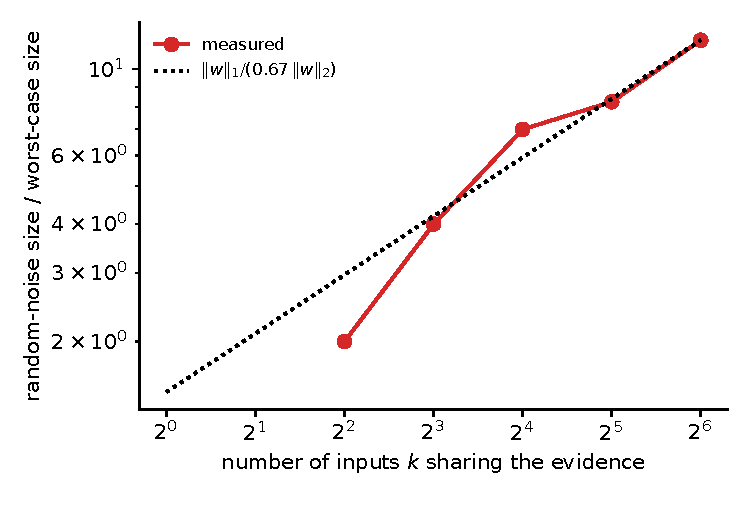
\includegraphics[width=0.5\textwidth]{h8_noise.pdf}
\caption{How many times larger random noise must be than the worst case to flip the answer, against the number of inputs $k$ sharing the evidence. Dotted: $\|w\|_1/(0.67\|w\|_2)$.}
\label{fig:h8}
\end{figure}

The gap grows like $\sqrt k$ (about $2$ at $k=4$, $12$ at $k=64$) and follows $\|w\|_1/\|w\|_2$.

\plain{Not a separate cause but the same one seen from another side: the more inputs share the evidence, the more the worst case beats random noise. No training is involved.}

\subsection{H10: the inevitable ceiling and the avoidable gap}
\label{sec:h10}

Here we ask directly how much vulnerability is inevitable. For a linear rule with weights $w$ the accuracy under the worst change of size $\epsilon$ is exactly $\Phi\big((\tfrac12\sum_i w_i\Delta\mu_i-\epsilon\|w\|_1)/\sqrt{\sum_i w_i^2\sigma_i^2}\big)$ ($\Delta\mu_i$ the class gap, $\sigma_i$ the noise of input $i$). We maximise it over $w$ at each $\epsilon$ to get the best accuracy under attack that any linear rule can reach (Figure~\ref{fig:h10}).

\begin{figure}[H]
\centering
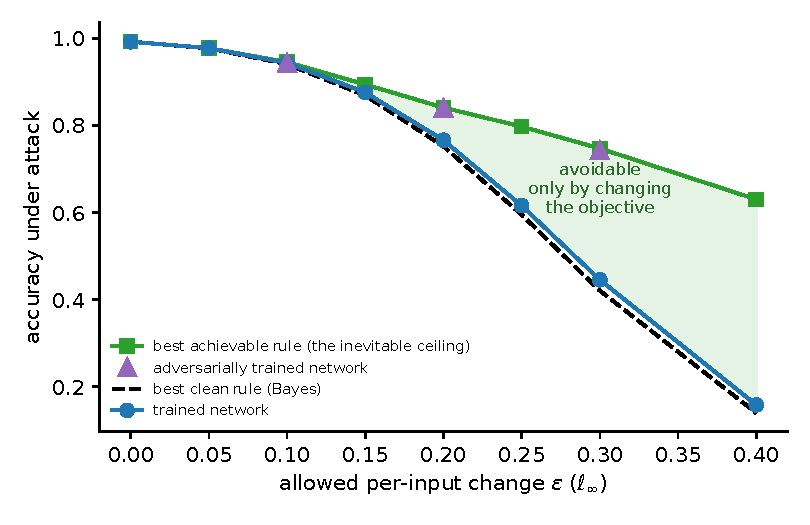
\includegraphics[width=0.62\textwidth]{h10_ceiling.pdf}
\caption{Accuracy under attack against the allowed per-input change. Green: the best achievable rule (the inevitable ceiling). Blue: a trained network. Purple triangles: the same network adversarially trained. Dashed: the best clean rule. The shaded gap is avoidable, but only by changing the training objective.}
\label{fig:h10}
\end{figure}

At $\epsilon=0.3$ the ceiling is $0.75$ (reached by using the reliable clue only), while the best clean rule gets $0.42$ and the trained network $0.45$. The ceiling itself falls as $\epsilon$ grows ($0.63$ at $\epsilon=0.4$): part of the loss is inevitable. The gap between ceiling and network, about $0.3$ at $\epsilon=0.3$, is avoidable, yet \emph{standard training will not close it}, because the standard objective rewards the clean-optimal rule. For small $\epsilon$ ($\le0.1$) the two coincide.

\paragraph{Does adversarial training close the gap?} We trained the same network by adversarial training (a 5-step attack on every batch). At $\epsilon=0.3$ it reaches $0.743\pm0.011$ accuracy under attack, against a ceiling of $0.748$ and $0.44$ for standard training; at $\epsilon=0.2$ it reaches $0.840$ against a ceiling of $0.841$ (standard: $0.76$); at $\epsilon=0.1$ there is no gap to close. The price is clean accuracy: $0.954$ and $0.960$ against $0.993$ (Figure~\ref{fig:h10}, triangles).

\plain{Both parts are real. The ceiling is inevitable. The gap is avoidable by changing the objective, and adversarial training closes it completely here, at the cost of the clean accuracy the weak clues carried: the accuracy/robustness trade-off of Tsipras et al.~\cite{tsipras2019} in numbers. The ceiling is for linear rules only.}

\subsection{H7: which solution the optimiser reaches}
\label{sec:h7}

Gradient descent on separable data is known to head for the solution with the largest margin measured in $\ell_2$, not in $\ell_\infty$ (Soudry et al.~\cite{soudry2018}). \textbf{Experiment:} 100 inputs, $s$ of them informative, 60 training examples (so the data are separable). Compare the $\ell_2$ max-margin classifier (we use an SVM as the stand-in for the gradient-descent limit) with the $\ell_\infty$ max-margin classifier (a linear programme) and the oracle best rule (Figure~\ref{fig:h7}).

\begin{figure}[H]
\centering
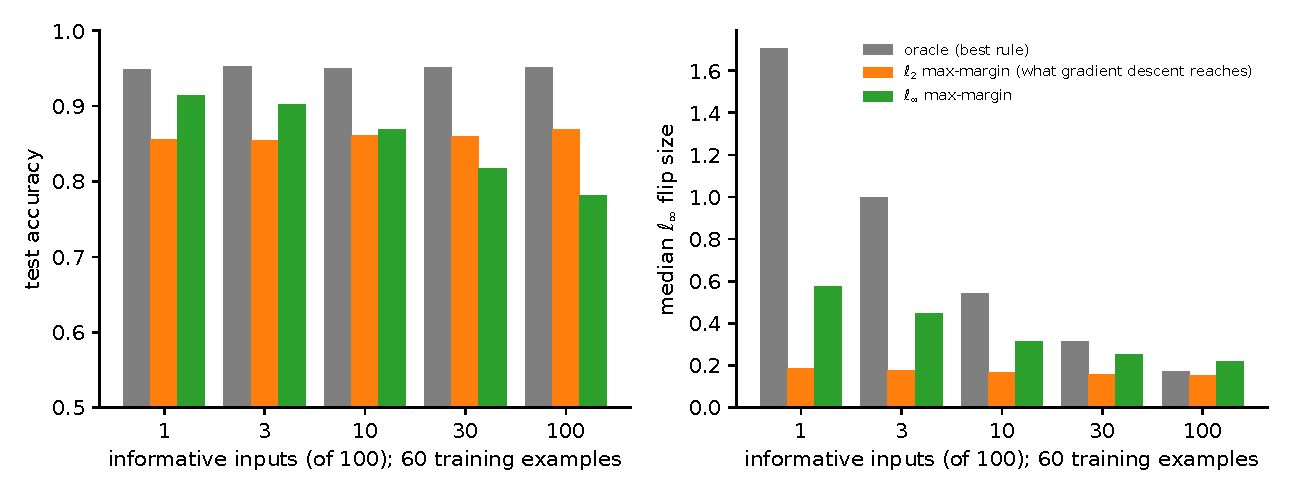
\includegraphics[width=0.98\textwidth]{h7_margin.pdf}
\caption{Accuracy (left) and per-input flip size (right) of three linear classifiers, against the number of informative inputs. The $\ell_\infty$ max-margin solution beats the $\ell_2$ one when the signal is sparse.}
\label{fig:h7}
\end{figure}

Figure~\ref{fig:illc} shows the two solutions on a few points in two dimensions: the $\ell_2$ solution tilts to use the irrelevant input, the $\ell_\infty$ solution does not.

\begin{figure}[H]
\centering
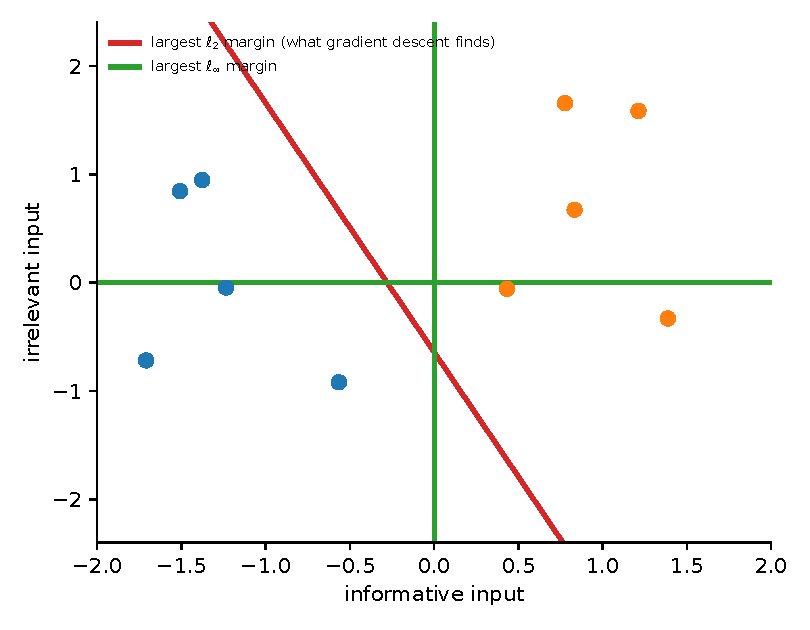
\includegraphics[width=0.5\textwidth]{ill_c_margin.pdf}
\caption{Ten training points; one input is informative, one irrelevant. Red: the largest-$\ell_2$-margin separator, the solution gradient descent reaches. Green: the largest-$\ell_\infty$-margin separator, which ignores the irrelevant input.}
\label{fig:illc}
\end{figure}

With a sparse signal ($s=1$) the $\ell_\infty$ solution is better on both axes (accuracy $0.92$ against $0.86$; flip size $0.57$ against $0.19$). With a dense signal the gap closes, and the $\ell_\infty$ solution then trades accuracy ($0.78$ against $0.87$) for a larger flip size ($0.22$ against $0.15$).

We checked the stand-in directly: 20\,000 steps of gradient descent on the logistic loss from zero end in a direction with cosine similarity $0.98$ to the SVM solution, with accuracy and flip size within about $0.015$ of it (for $s=1$: accuracy $0.869$ against $0.855$, flip size $0.199$ against $0.186$).

\plain{The optimiser's bias towards $\ell_2$ is an avoidable contribution when the truth is sparse and data are scarce. When the truth is dense, the gap is the trade-off again.}

\subsection{H6: more data}
\label{sec:h6}

\textbf{Claim} (Schmidt et al.~\cite{schmidt2018}): robust generalisation needs more data. \textbf{Experiment (standard training only):} train on $n=30$ to $4000$ examples, with the evidence spread over 16 inputs (Figure~\ref{fig:h6}).

\begin{figure}[H]
\centering
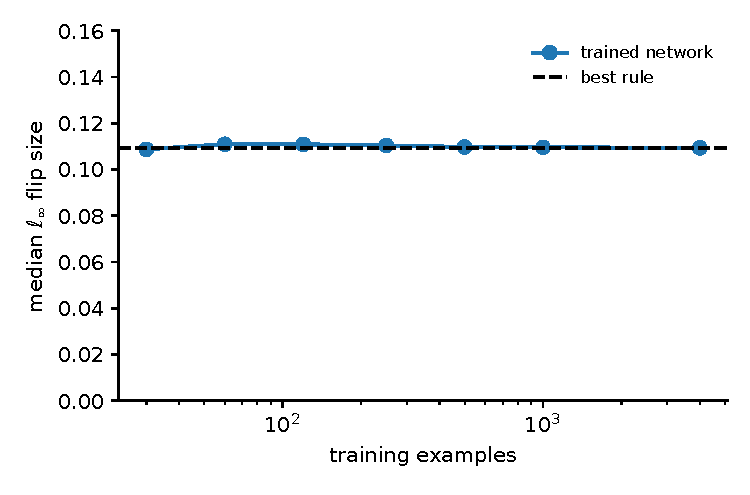
\includegraphics[width=0.5\textwidth]{h6_data.pdf}
\caption{Per-input flip size against the number of training examples. The trained network matches the best rule at every $n$.}
\label{fig:h6}
\end{figure}

Accuracy rises from $0.905$ to $0.953$, but the flip size equals the best rule's ($0.109$--$0.111$) at every $n$.

\paragraph{With adversarial training.} Schmidt et al.'s claim is about robust (adversarially trained) learning, so we repeat the experiment with it. In the toy world with $64$ inputs ($\epsilon=0.03$, ceiling $0.76$), adversarial and standard training give the same accuracy under attack at every $n$, both climbing to the ceiling ($0.62$ at $n=30$, $0.75$ at $n=1000$, $0.76$ at $n=16\,000$). The data needed to get within a few percent of the ceiling grows with the number of inputs: about $100$ examples with $16$ inputs, about $1000$ with $64$. On real data (Figure~\ref{fig:atdata}), standard networks have almost no accuracy under attack at any size (MNIST $0.01$--$0.05$, CIFAR-10 $0.03$--$0.06$), while adversarially trained ones reach $0.25$, $0.57$, $0.69$ (MNIST, $\epsilon=0.1$, $100$, $1000$, $10\,000$ examples) and $0.22$, $0.47$, $0.57$ (CIFAR-10, $\epsilon=2/255$, $1000$, $5000$, $20\,000$ examples). Their flip sizes are $1.5$--$3\times$ (MNIST) and $2$--$6\times$ (CIFAR-10) those of standard networks, at a clean-accuracy cost of up to $6$ points on CIFAR-10 and about $0$--$1$ points on MNIST (where the cost is negative at $1000$ examples).

\begin{figure}[H]
\centering
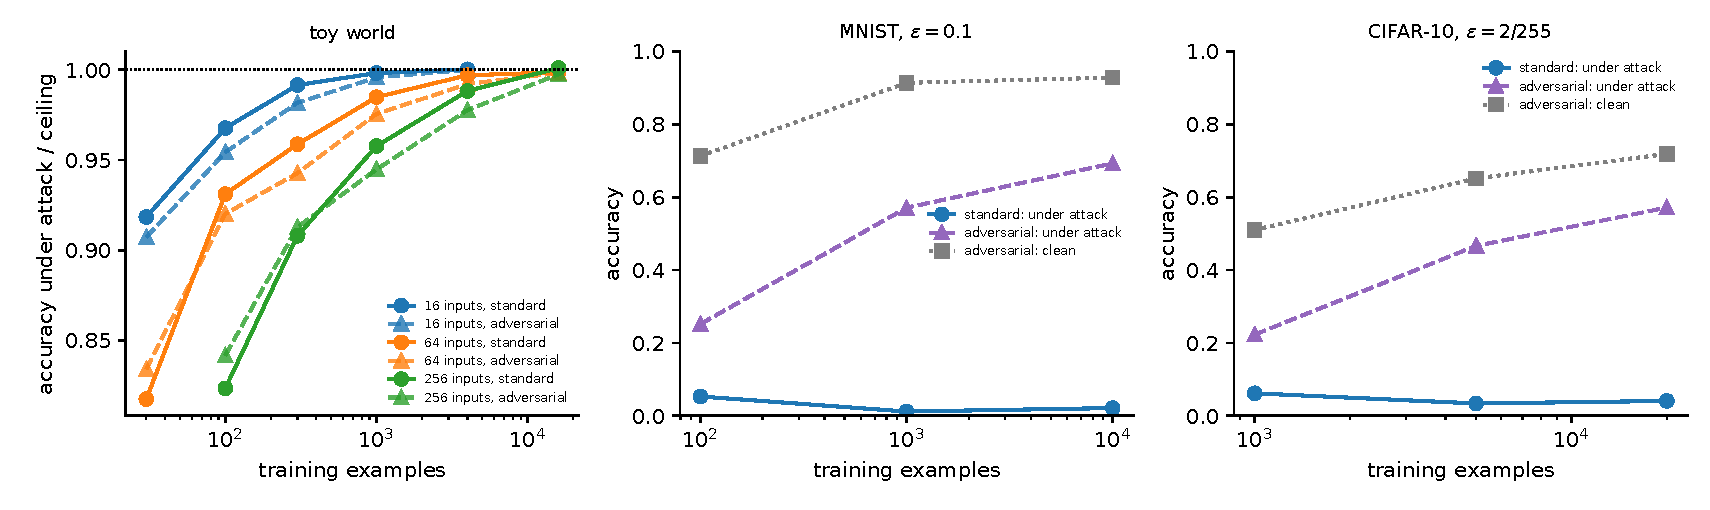
\includegraphics[width=0.98\textwidth]{at_data.pdf}
\caption{Accuracy under attack against the number of training examples, with standard and adversarial training. Left: the toy world with $64$ inputs (dotted: the ceiling). Middle and right: MNIST and CIFAR-10; the dotted gray line is the clean accuracy of the adversarially trained network.}
\label{fig:atdata}
\end{figure}

\plain{Under standard training, more data does not change vulnerability, in the toy world or on real data. Under adversarial training, data quantity matters a lot for real data (robust accuracy rises steeply with $n$), as Schmidt et al.\ argue; in the toy world adversarial training needs no more data than standard training to reach the same ceiling, though the data needed grows with the number of inputs. So data quantity is a cause of \emph{robust learning being hard}, not of standard models being fragile.}

\subsection{H5: directions the data never use}
\label{sec:h5}

\textbf{Claim} (Gilmer et al.~\cite{gilmer2018}; Stutz et al.~\cite{stutz2019}): networks are sensitive in directions off the data manifold, where training gives no signal. \textbf{Experiment:} data lie on a 4-dimensional subspace of a 64-dimensional space (plus small off-subspace noise). Attack only along the subspace, or only across it (Figure~\ref{fig:h5}).

\begin{figure}[H]
\centering
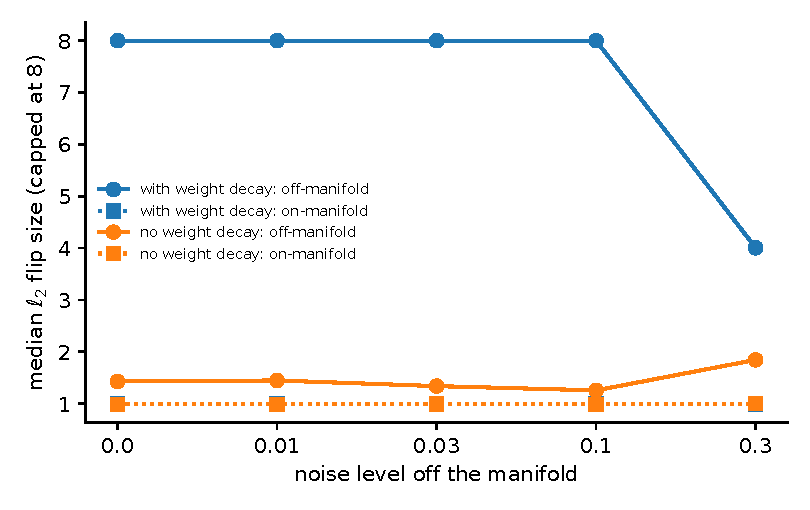
\includegraphics[width=0.55\textwidth]{h5_manifold.pdf}
\caption{Median total flip size when the attack is limited to the data subspace (squares) or to the directions across it (circles), with and without weight decay. Values above $8$ are shown as $8$ (no flip found).}
\label{fig:h5}
\end{figure}

With weight decay the network ignores off-manifold directions entirely (no flip found within $8$). Without weight decay, off-manifold flip sizes are $1.3$--$1.8$, close to the on-manifold $1.0$, and an attack free to use both is about $20\%$ stronger than one limited to the subspace.

\plain{Real but modest, and \emph{avoidable}: the best rule is blind to these directions and ordinary weight decay makes the network blind too. Contributes; not the main cause here.}

\subsection{H3: shape versus texture}
\label{sec:h3}

\textbf{Claim} (Geirhos et al.~\cite{geirhos2019}; for frequency, Yin et al.~\cite{yin2019}): networks lean on texture (fine, high-frequency patterns) more than people do, and texture reliance makes them fragile. \textbf{World:} $16\times16$ images with Gaussian pixel noise. A cue is a fixed pattern added with a class-dependent sign; its strength, and hence the accuracy it supports ($\approx95\%$), is set exactly (Figure~\ref{fig:illd}).

\begin{figure}[H]
\centering
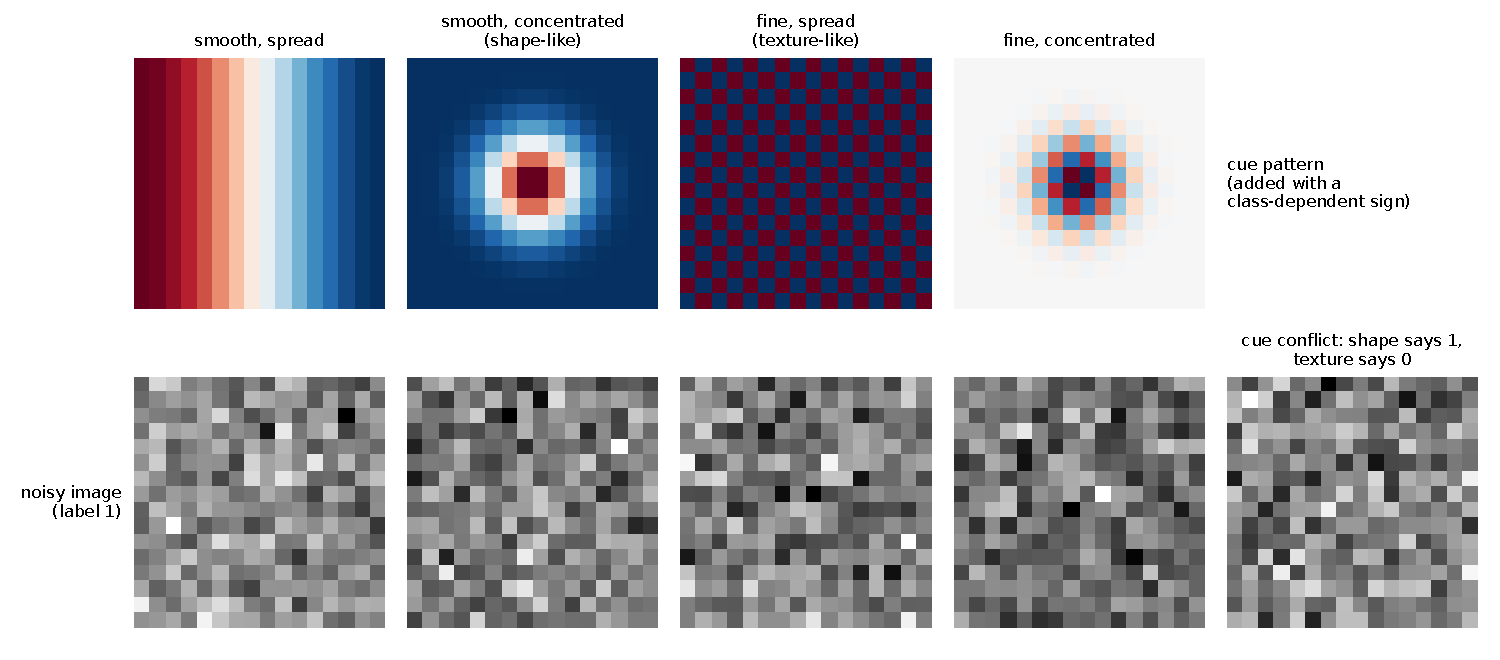
\includegraphics[width=0.95\textwidth]{ill_d_cues.pdf}
\caption{The cues. Top: the four patterns (red positive, blue negative); the first three are used in experiment 1, the first and third in experiment 2. Bottom: the same patterns at the strength used, buried in pixel noise, and a cue-conflict image in which the shape cue says class 1 and the texture cue says class 0.}
\label{fig:illd}
\end{figure}

\paragraph{Experiment 1: frequency or spread?} Four cues of equal strength: \emph{smooth} or \emph{fine} (a checkerboard), each \emph{spread} over the whole image or \emph{concentrated} in the middle. We report the cue's spread as the $\ell_1/\ell_2$ ratio of its pattern ($14.4$, $7.1$, $16.0$, $7.1$); Figure~\ref{fig:h3} (left) shows the results.

\begin{figure}[H]
\centering
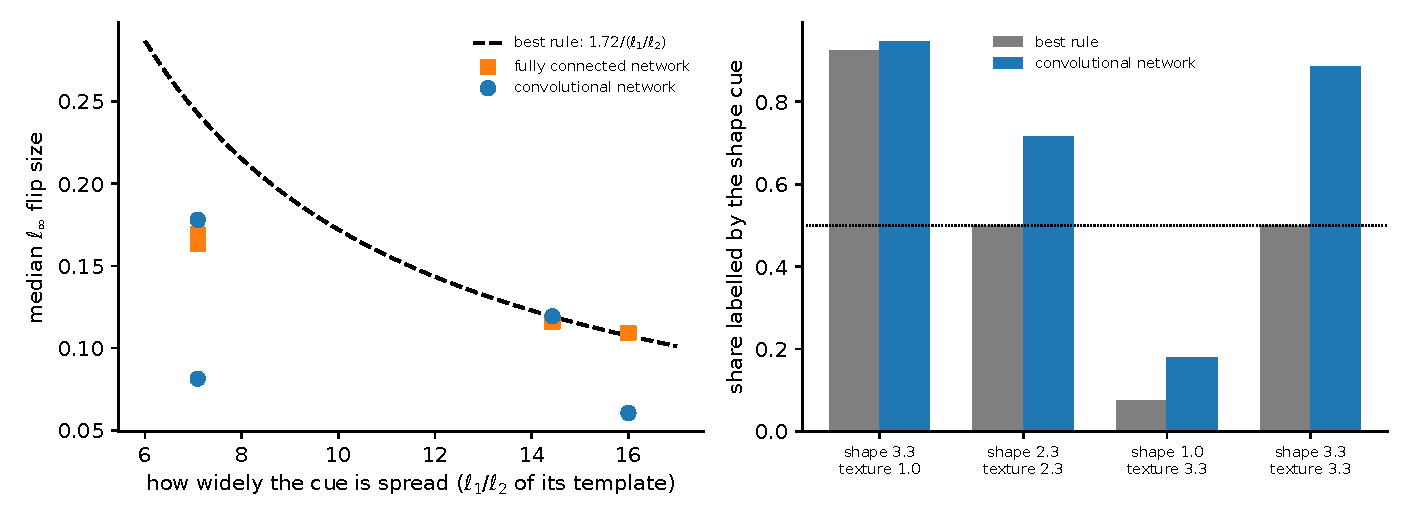
\includegraphics[width=0.98\textwidth]{h3_shape_texture.pdf}
\caption{Left: per-input flip size of the best rule (dashed), a fully connected network (squares) and a convolutional network (circles) for four cues of equal strength, against how widely the cue is spread. Right (experiment 2): in images where the shape cue and the texture cue disagree, the share labelled by the shape cue, for the best rule and the convolutional network.}
\label{fig:h3}
\end{figure}

For the best rule, flip size times spread is the same for all four cues ($1.70$--$1.73$, equal to the total flip size): \emph{frequency does not matter; spread does}. The fully connected network follows the best rule on the spread cues ($0.116$ against $0.120$; $0.109$ against $0.107$) and is $1.45\times$ more fragile on the concentrated ones ($0.163$ against $0.240$; $0.169$ against $0.242$), the same effect as in H4a. The convolutional network (two convolution--ReLU--max-pool stages) matches the best rule on the smooth cues but not on the fine ones: accuracy falls to $0.87$ and $0.86$ and the flip size to $0.06$ and $0.08$ (best rule $0.11$ and $0.24$), and even the total flip size drops ($0.72$ against $1.7$).

\paragraph{Experiment 2: cue conflict.} Images carry both a shape-like cue (smooth, concentrated) and a texture-like cue (fine, spread). In test images the two disagree. The best rule follows whichever cue is stronger, and is indifferent at equal strength. The convolutional network follows the stronger cue too, but at equal strength it is \emph{shape-biased}: it follows the shape cue in $72\%$ and $89\%$ of images for equal strengths $2.3$ and $3.3$. Flip sizes follow what the model relies on: $0.19$ when the shape cue dominates (strengths $3.3$ and $1.0$) and $0.067$ when the texture cue does ($1.0$ and $3.3$), $2.8\times$ more fragile (the spread ratio is $2.3$). A worst-case change puts its energy along the cue the model uses (fraction along the shape template $0.39$ against $0.03$ along the texture template when shape dominates; $0.10$ against $0.33$ when texture dominates).

\plain{``Texture'' as a category is not a separate cause. For the best rule only spread matters, so a fine pattern is fragile when it is spread over many pixels and not otherwise. Trained networks add architecture-specific effects: this convolutional network reads fine patterns badly (avoidable) and prefers shape at equal strength. Caveat: a $16\times16$ toy and one architecture; the real-data check is still to do.}

\subsection{H9: architecture and invariance}
\label{sec:h9}

\textbf{Question:} does building in the right invariance reduce vulnerability, or only move it? \textbf{World:} $16\times16$ noisy images; the label is whether a small known pattern ($3\times3$ block) is present \emph{anywhere} (Figure~\ref{fig:ille}). We compare a fully connected network, a small translation-invariant convolutional network (convolution plus a global maximum), and the hand-built matched filter, which knows the pattern (results in Figure~\ref{fig:h9}).

\begin{figure}[H]
\centering
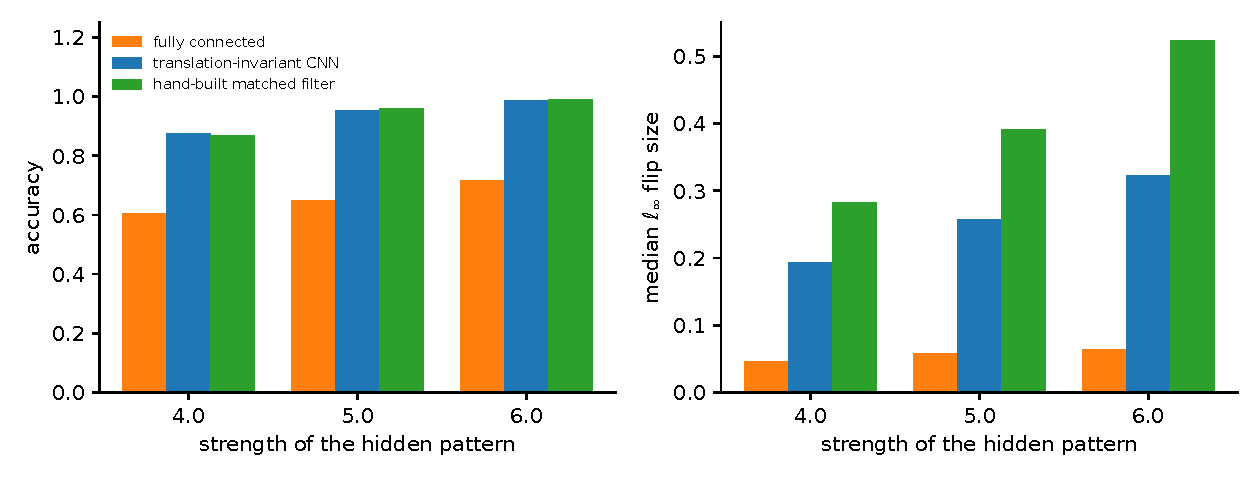
\includegraphics[width=0.98\textwidth]{h9_invariance.pdf}
\caption{Accuracy (left) and per-input flip size (right) against the strength of the hidden pattern, for three models (3 runs).}
\label{fig:h9}
\end{figure}

\begin{figure}[H]
\centering
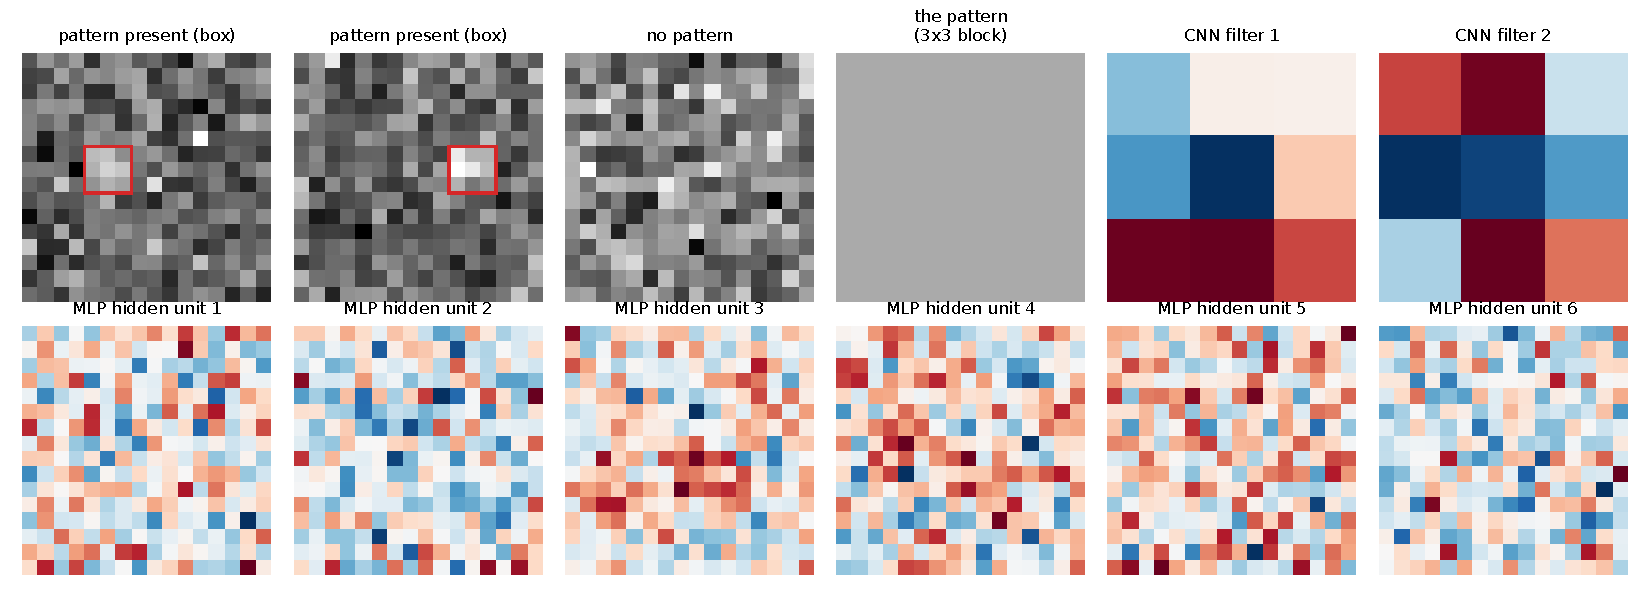
\includegraphics[width=0.98\textwidth]{ill_e_invariance.pdf}
\caption{The invariance task and what is learned. Top: images with and without the hidden pattern (red box: where the matched filter finds it), the pattern, and two filters learned by the convolutional network (they resemble the pattern). Bottom: the input weights of six hidden units of the fully connected network, which show no pattern: it has to learn each position separately.}
\label{fig:ille}
\end{figure}

Figure~\ref{fig:h9} shows the result. The right invariance helps on both axes: at strength $6$ the convolutional network reaches accuracy $0.99$ with flip size $0.32$, while the fully connected network (data-starved with $3000$ examples) reaches $0.72$ with $0.064$. But the learned convolutional network is still about $1.6\times$ more fragile than the matched filter at the same accuracy ($0.32$ against $0.52$ at strength $6$; $0.19$ against $0.28$ at strength $4$). We have not diagnosed why.

\plain{The right inductive bias reduces vulnerability substantially, but a learned solution does not reach the best hand-built one at equal accuracy: an avoidable gap remains. Caveat: the fully connected network is not at equal accuracy, so its flip size mixes data hunger with fragility.}

\section{Do the toy findings survive on real images?}
\label{sec:real}

Each toy hypothesis that can be checked without adversarial training gets a real-data counterpart. Data: MNIST and Fashion-MNIST (small fully connected network) and CIFAR-10 (small convolutional network), $10\,000$ training images, standard training, flip sizes over $300$ test images, 2--3 runs (settings in Appendix~\ref{app:settings}). The ceiling experiment (H10) needs the unknown best robust classifier and is not repeated. Figures~\ref{fig:reala} and~\ref{fig:realb} and Table~\ref{tab:real} summarise the results.

\begin{figure}[H]
\centering
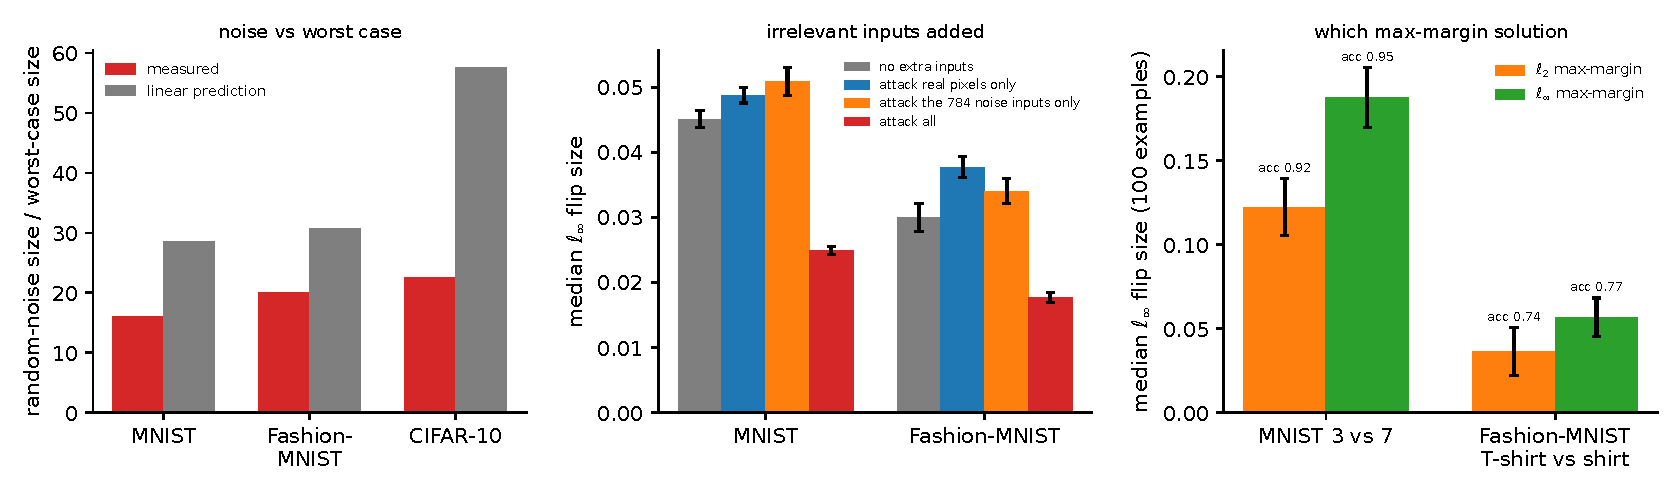
\includegraphics[width=0.98\textwidth]{real_a.pdf}
\caption{Real-data counterparts of H8, H4a and H7. Left: how many times larger random noise must be than the worst case, measured and as predicted by the linear picture. Middle: flip size after appending $784$ irrelevant noise inputs to each image. Right: $\ell_\infty$ flip size and accuracy of the two max-margin solutions trained on $100$ examples.}
\label{fig:reala}
\end{figure}

\paragraph{H8, noise versus the worst case.} Random noise must be $16\times$ (MNIST), $20\times$ (Fashion-MNIST) and $24\times$ (CIFAR-10) larger than the worst case to flip a quarter of the points. The linear prediction ($\ell_2$ flip size over $\ell_\infty$ flip size over $0.67$) gives $29$, $31$ and $56$: the right order of magnitude, overestimating by $1.3$--$2.3\times$. On CIFAR-10 random noise of size $0.076$ is needed against $0.003$ for the worst case.

\paragraph{H4a, irrelevant inputs.} We append $784$ pure-noise inputs to every image. Attacking only the real pixels flips at $0.049$ (without extra inputs: $0.045$), attacking only the noise inputs flips at $0.050$, and attacking everything at $0.025$. The network is as sensitive to inputs that carry no information as to real ones, and the combined flip size is $1.8\times$ smaller (Fashion-MNIST: $0.037$, $0.034$, $0.018$). This reproduces the toy factor of about two. Figure~\ref{fig:illf} shows why: the network's gradient with respect to the 784 irrelevant inputs is as large in total as its gradient with respect to the real pixels.

\begin{figure}[H]
\centering
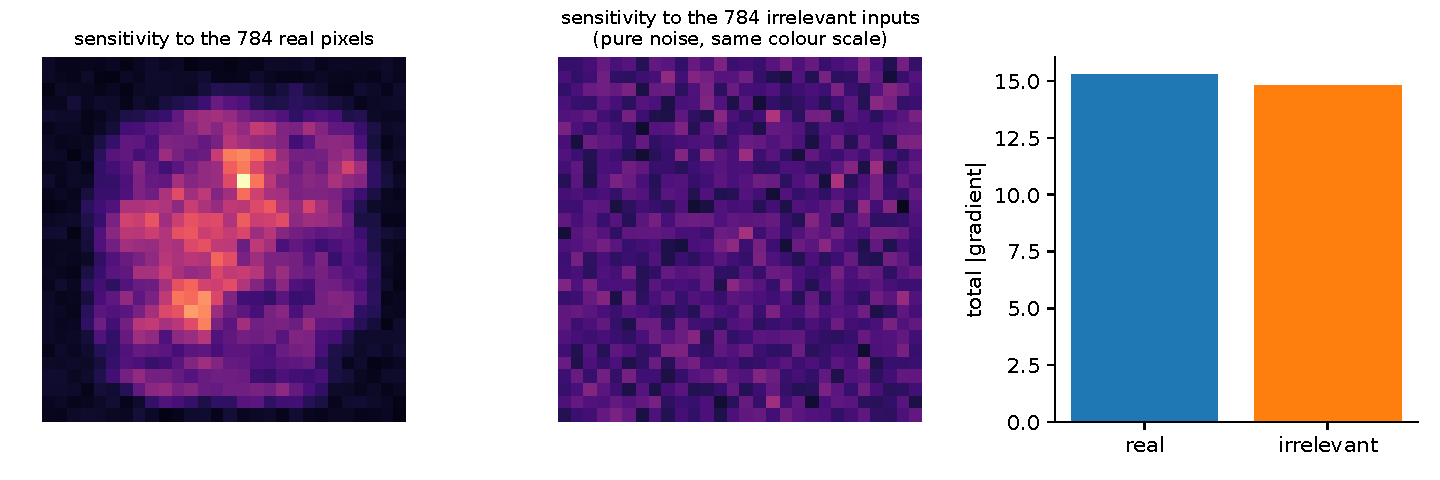
\includegraphics[width=0.95\textwidth]{ill_f_irrelevant.pdf}
\caption{Average size of the loss gradient of the network trained with $784$ appended irrelevant inputs, over $500$ test images: real pixels (left), irrelevant inputs on the same colour scale (middle), and their totals (right).}
\label{fig:illf}
\end{figure}


\paragraph{H7, which solution.} The $\ell_\infty$ max-margin classifier beats the $\ell_2$ one on both accuracy and flip size at every training size we tried ($40$, $100$, $300$) on MNIST (3 versus 7) and Fashion-MNIST (T-shirt versus shirt). With $100$ examples: MNIST accuracy $0.954$ against $0.919$ and flip size $0.188$ against $0.122$ ($+54\%$); Fashion-MNIST $0.771$ against $0.735$ and $0.057$ against $0.036$ ($+58\%$). (The SVM's accuracy on MNIST dips at $300$ examples, $0.886$, which may be solver tolerance.)

\begin{figure}[H]
\centering
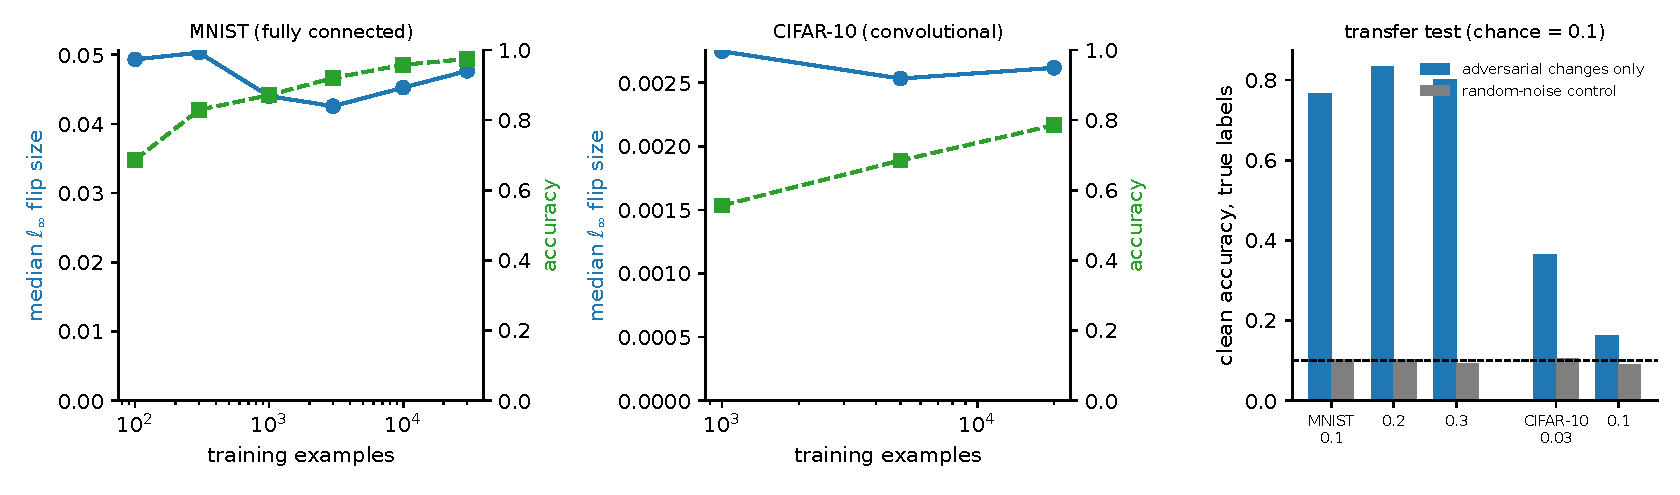
\includegraphics[width=0.98\textwidth]{real_b.pdf}
\caption{Left and middle (H6): flip size (blue) and accuracy (green) against the number of training examples, for MNIST and CIFAR-10. Right (H2): clean accuracy of a fresh network trained only on adversarially changed images with random target labels (blue) against a random-noise control, for the sizes of change shown (chance $=0.1$).}
\label{fig:realb}
\end{figure}

\paragraph{H2, transfer.} A fresh network trained only on adversarially changed images with random target labels reaches clean accuracy $0.77$, $0.83$ and $0.80$ on MNIST for changes of size $0.1$, $0.2$ and $0.3$, and $0.37$ on CIFAR-10 at $0.03$ ($0.16$ at $0.1$); the random-noise controls stay at chance ($\approx0.10$). Adversarial changes carry learnable features on real data too, much more weakly on CIFAR-10 with these small networks. Figure~\ref{fig:illi} shows how the training data for this test look.

\begin{figure}[H]
\centering
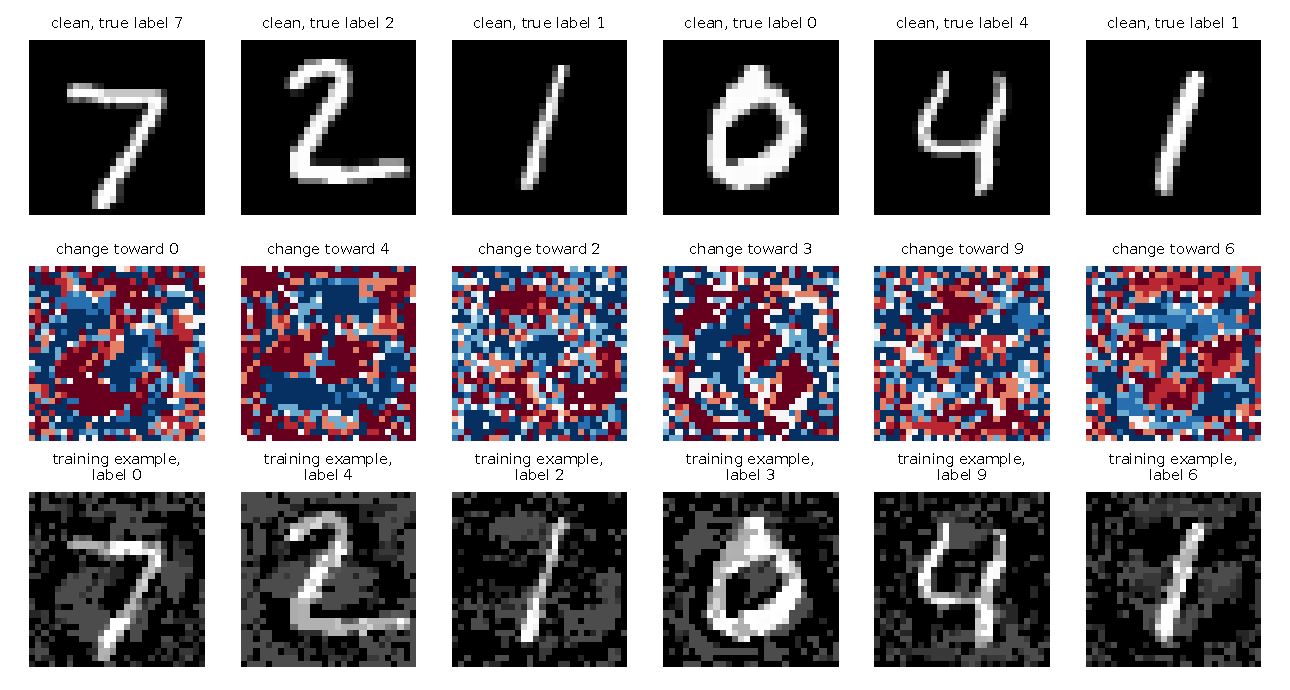
\includegraphics[width=0.8\textwidth]{ill_i_transfer.pdf}
\caption{Building the transfer test on MNIST. Top: a clean image and its true label. Middle: the targeted change ($\epsilon=0.3$) towards a random other label. Bottom: the training example, an image that looks like the original digit but carries the target label.}
\label{fig:illi}
\end{figure}


\paragraph{H6, more data.} On MNIST the flip size is flat ($0.043$--$0.050$, Figure~\ref{fig:realb}) from $100$ to $30\,000$ examples while accuracy rises from $0.69$ to $0.97$. On CIFAR-10 it is flat too ($0.0027$, $0.0025$, $0.0026$ for $1000$, $5000$, $20\,000$ examples; accuracy $0.56$, $0.69$, $0.79$) once every training-set size gets the same number of optimiser steps. (A first run with a fixed number of epochs showed a flip size falling with data; that was an artefact of undertraining the small sets.)

\begin{table}[H]
\centering
\caption{Real-data checks of H5, H3 and H9. Median flip sizes ($\ell_2$ for the subspace and band rows). PC = principal component.}
\label{tab:real}
\small
\resizebox{\textwidth}{!}{%
\begin{tabular}{llcccc}
\toprule
Check & Data & Condition A & Condition B & Unrestricted & Accuracy \\
\midrule
H5: attack on / off the top PCs & MNIST (50 PCs) & on: $1.08$ & off: $1.42$ & $0.87$ & $0.96$ \\
 & CIFAR-10 (200 PCs) & on: $0.47$ & off: $0.12$ & $0.11$ & $0.73$ \\
H3: lowest / highest 25\% of frequencies & MNIST & low: $0.97$ & high: $4.41$ & $0.87$ & $0.96$ \\
 & CIFAR-10 & low: $0.27$ & high: $0.32$ & $0.12$ & $0.73$ \\
H9: fully connected / convolutional ($\ell_\infty$) & MNIST & $0.045$ & $0.088$ & -- & $0.96$ / $0.98$ \\
 & Fashion-MNIST & $0.030$ & $0.029$ & -- & $0.85$ / $0.87$ \\
 & CIFAR-10 & $0.0052$ & $0.0032$ & -- & $0.46$ / $0.73$ \\
\bottomrule
\end{tabular}}
\end{table}

\paragraph{H5, off-manifold.} On MNIST the network is \emph{less} sensitive off the top $50$ components (flip size $1.42$) than along them ($1.08$), with or without weight decay. On CIFAR-10 it is four times more sensitive off the top $200$ components ($0.12$ against $0.47$), and an unrestricted attack is no stronger than the off-subspace one ($0.11$). Caveat: the off-subspace has about $14\times$ more directions than the subspace. Figure~\ref{fig:illg} shows the smallest change that flips one image, split into its part along the top components and the rest: on MNIST $72\%$ of its energy lies along the top $50$ components, on CIFAR-10 only $7\%$ lies along the top $200$.

\begin{figure}[H]
\centering
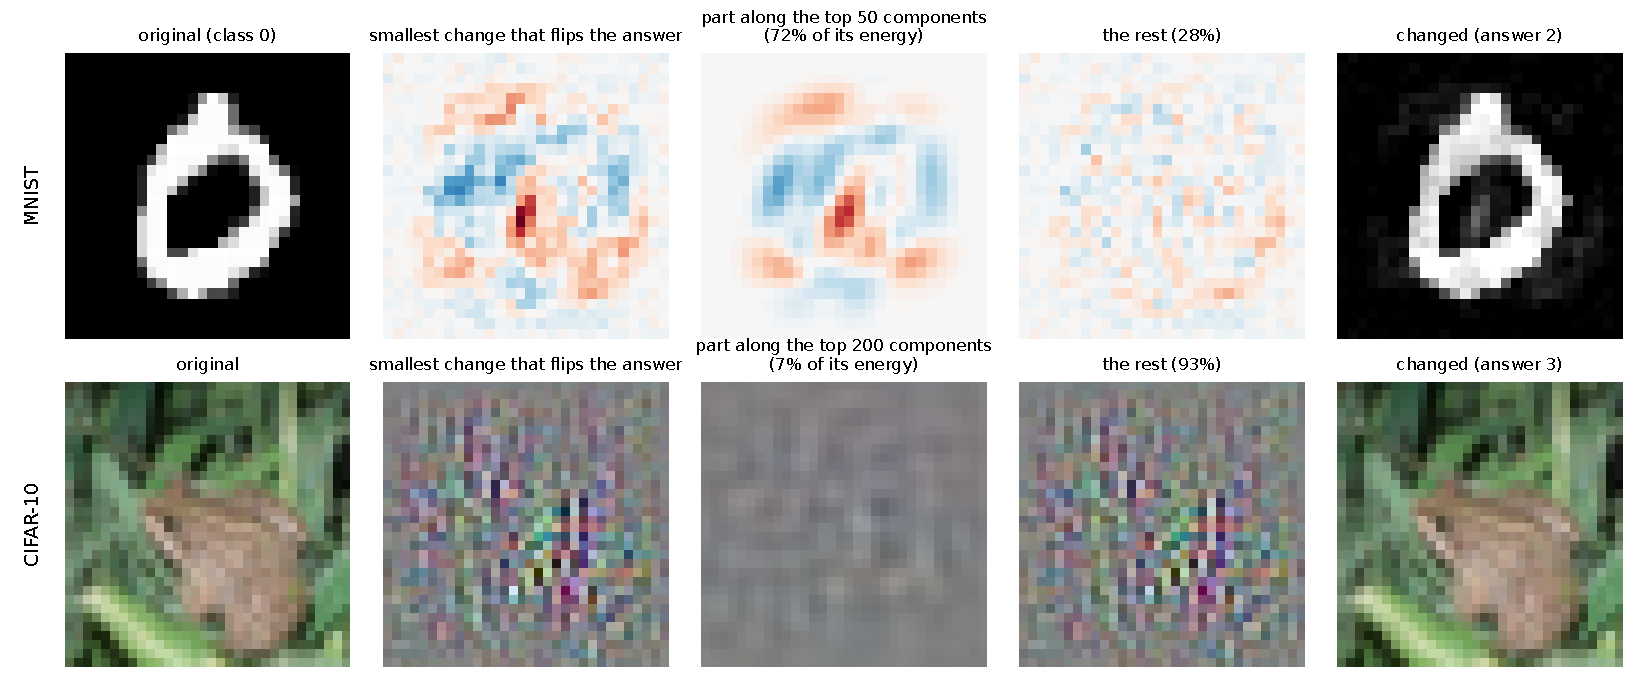
\includegraphics[width=0.98\textwidth]{ill_g_where.pdf}
\caption{Where the smallest flipping change goes. Columns: the original image, the smallest total ($\ell_2$) change that flips the answer (scaled for visibility), its part along the top principal components, the remainder, and the changed image with the new answer.}
\label{fig:illg}
\end{figure}


\paragraph{H3, frequency.} Restricting the change to the lowest or highest quarter of the frequencies, the network shows no special fragility to high frequencies: on MNIST it is far \emph{less} sensitive to them ($4.4$ against $1.0$), on CIFAR-10 about equally sensitive ($0.32$ against $0.27$).

\paragraph{H9, architecture.} The convolutional network doubles the $\ell_\infty$ flip size on MNIST ($0.088$ against $0.045$) but is no better on Fashion-MNIST, and on CIFAR-10 it is more accurate ($0.73$ against $0.46$) but has a \emph{smaller} flip size ($0.0032$ against $0.0052$).

\paragraph{Larger networks.} To check that the small networks are not the reason, we repeat the main checks with a $1024$-unit, four-layer fully connected network on MNIST and a ResNet-18 on CIFAR-10 (Table~\ref{tab:big}).

\begin{table}[H]
\centering
\caption{Larger networks. Median flip sizes ($\ell_\infty$ unless marked $\ell_2$); same conditions as the small networks.}
\label{tab:big}
\small
\resizebox{\textwidth}{!}{%
\begin{tabular}{lcc}
\toprule
Check & Wide MLP, MNIST & ResNet-18, CIFAR-10 \\
\midrule
Accuracy ($10\,000$ / $20\,000$ images) & $0.962$ & $0.809$ \\
$\ell_\infty$ flip size (small network) & $0.044$ ($0.045$) & $0.0039$ ($0.0032$) \\
H6: flip size at $n=100$ / $1000$ / $10\,000$ / $60\,000$ (MNIST), $n=1000$ / $5000$ / $20\,000$ (CIFAR-10) & $0.038$, $0.038$, $0.044$, $0.052$ & $0.0027$, $0.0046$, $0.0039$ \\
H4a: attack real / noise inputs / all (flip size without noise inputs) & $0.045$ / $0.048$ / $0.024$ ($0.044$) & -- \\
H5: $\ell_2$ flip size on / off the top PCs (unrestricted) & $1.11$ / $1.38$ ($0.87$) & $0.47$ / $0.16$ ($0.16$) \\
H3: $\ell_2$ flip size, lowest / highest 25\% of frequencies & $0.98$ / $3.87$ & $0.31$ / $0.60$ \\
\bottomrule
\end{tabular}}
\end{table}

The picture does not change. Irrelevant inputs halve the flip size again ($1.8\times$). Flip size is flat in the amount of data on MNIST and varies by less than $1.7\times$ without trend on CIFAR-10. Off-manifold sensitivity appears on CIFAR-10 ($3\times$) and not on MNIST. Neither network is more fragile at high frequencies (the ResNet is $1.9\times$ \emph{less} sensitive to them). The ResNet-18 has a slightly larger flip size than the small convolutional network at much higher accuracy ($0.81$ against $0.73$).

\plain{Real data mostly confirm the toy mechanisms and the avoidable effects: noise versus worst case (same order), irrelevant inputs (about $1.8\times$), optimiser bias ($+50\%$), and transfer. They qualify others: more data does not change standard flip sizes, off-manifold sensitivity is a CIFAR-10 effect, high-frequency fragility is not found, and a better architecture is not consistently more robust. Larger networks give the same picture. Caveats: few runs, one dataset per kind, standard training in these checks (adversarial training in Section~\ref{sec:h6}).}

Two earlier checks complete the picture. Mixing the pixels of MNIST digits with a random rotation (same information, same total distances) leaves total flip size unchanged but shrinks per-input flip size by only $12$--$14\%$, not the eightfold drop of the toy world: pixel data are already in the spread-out regime. On CIFAR-10, letting the network use more principal components raises accuracy ($44\%\to78\%$) and shrinks \emph{both} flip sizes by about $7$--$8\times$, so that loss is a shrinking margin, not spreading. A pilot comparing the networks with nearest-neighbour classifiers shows why ``a robust classifier exists'' is hard to establish in $\ell_\infty$ (compare the separation argument of Yang et al.~\cite{yang2020}): on raw pixels every pair of images is almost equally far apart (nearest same-class and other-class distances are both about $0.99$ on MNIST).

\section{Scorecard}
\label{sec:score}

Figure~\ref{fig:illj} gives the scorecard at a glance and Table~\ref{tab:score} the evidence behind it.


\begin{figure}[H]
\centering
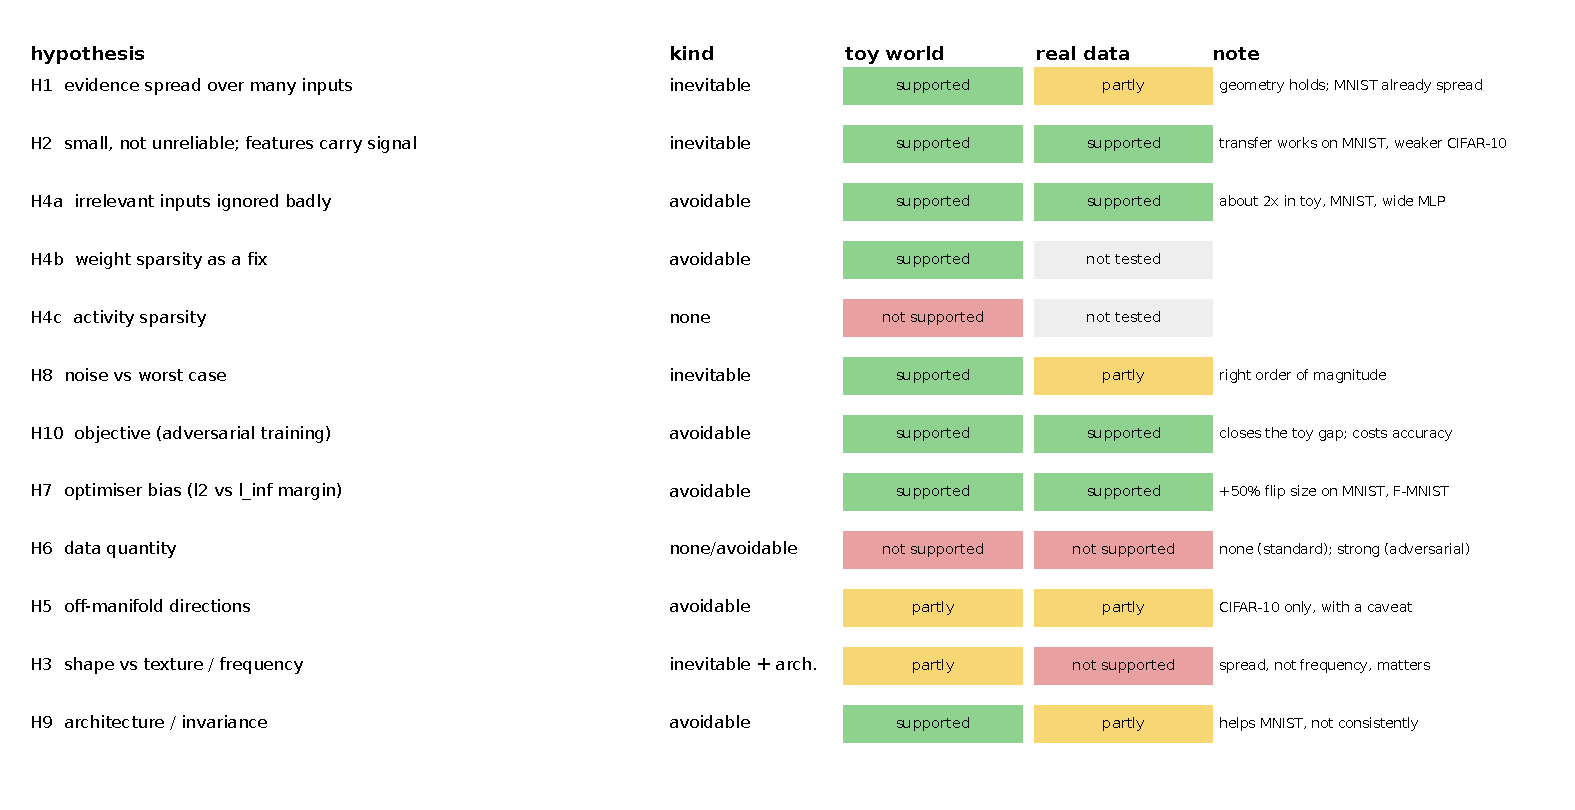
\includegraphics[width=0.98\textwidth]{ill_j_scorecard.pdf}
\caption{The scorecard at a glance. Green: supported; yellow: partly; red: not supported; gray: not tested. ``Kind'' is whether the effect is inevitable or avoidable.}
\label{fig:illj}
\end{figure}

\begin{table}[H]
\centering
\caption{Scorecard. ``Role'': necessary (N), sufficient (S), contributes (C), not supported (--). ``Kind'': inevitable (I) or avoidable (A).}
\label{tab:score}
\footnotesize
\begin{tabular}{p{2.3cm}p{1.0cm}p{1.0cm}p{4.7cm}p{4.7cm}}
\toprule
Hypothesis & Role & Kind & Toy world & Real data \\
\midrule
H1 evidence spread over many inputs & N, S & I & flip size $\propto1/\sqrt k$ exactly; absent under $\ell_2$ & geometry holds; MNIST already spread out; CIFAR-10 loss is margin \\
H2 small, not unreliable & N, S & I & flip size $\propto$ size; adversarial changes teach a fresh network the true classes (10/10) & transfer works: MNIST $0.77$--$0.83$, CIFAR-10 $0.37$ (chance $0.10$) \\
H4a dense signal / irrelevant inputs & S / C & I / A & dense: same as H1; network up to $2\times$ worse than best rule with irrelevant inputs & appended noise inputs: $1.8\times$ smaller flip size (MNIST), $1.7\times$ (Fashion-MNIST) \\
H4b weight sparsity & fix & A & removes fragility at an accuracy cost & not tested \\
H4c activity sparsity & -- & -- & no effect; fails all at once & not tested \\
H8 noise sensitivity & (H1) & I & restates H1: ratio $\propto\sqrt k$ & ratio $16$--$24$, linear prediction $29$--$56$ \\
H10 objective & C & A (new objective) & ceiling $0.75$ vs standard $0.45$ at $\epsilon=0.3$; adversarial training reaches $0.74$ & adversarial training: flip size $\times1.5$--$6$, clean accuracy up to $-6$ points (CIFAR-10), $\approx0$ (MNIST) \\
H7 optimiser bias & C & A & $\ell_\infty$ max-margin better when signal sparse, data scarce; gradient descent matches SVM & $\ell_\infty$ solution: $+54\%$ (MNIST), $+58\%$ (Fashion-MNIST) flip size, higher accuracy \\
H6 data quantity & -- (standard); C (adversarial) & A & no effect under standard training; adversarial training needs no more data than standard, but data needed grows with inputs & flat for standard training (small and large networks); adversarial robust accuracy rises $0.25\to0.69$ with data \\
H5 off-manifold & C (small) & A & vanishes with weight decay; $\sim20\%$ without & CIFAR-10: $3$--$4\times$ more sensitive off top PCs (small CNN, ResNet-18); MNIST: not \\
H3 shape vs texture & C & I, A & spread is inevitable (best rule: flip size $\times$ spread constant, frequency irrelevant); architecture is avoidable (CNN weak on fine patterns, shape-biased) & no special high-frequency fragility (MNIST less, CIFAR-10 equal) \\
H9 architecture & C & A & invariance: $4$--$5\times$ flip size over fully connected, $1.6\times$ below hand-built filter & MNIST $2\times$ better; Fashion-MNIST equal; CIFAR-10 smaller flip size \\
\bottomrule
\end{tabular}
\end{table}

\section{Discussion (draft)}

In the toy worlds, the first-order cause of fragility to small per-input changes is inevitable: the evidence a good classifier uses is spread over many inputs or carried by clues that are small compared with the allowed change, and a per-input budget lets the attacker push all of it together. Several explanations that look different (noise sensitivity, dense signals, texture reliance as a category) are the same mechanism seen from other sides: only how widely the evidence is spread matters for the best rule. Avoidable causes exist and can be sizeable (up to a factor of two from ignoring irrelevant inputs; $1.6\times$ from a learned rather than designed filter; a convolutional network that reads fine patterns badly; large when the objective ignores robustness), but they sit on top of the inevitable one and cannot remove it. The real-data checks, with small and large networks, support the mechanism and several of the avoidable effects (irrelevant inputs, optimiser bias, transfer, the objective) but not every toy prediction (off-manifold sensitivity, architecture). So this remains a hypothesis about large networks, not a result.

\paragraph{What would change our mind.} A real task where the classes are well separated in $\ell_\infty$, a robust classifier is easy to write down, and standard training still finds a fragile one, would be a case where the avoidable part dominates. Finding or constructing such a case on real data is the most valuable open test.

\section{Limits}

Independent Gaussian clues, small networks, one-step and projected attacks, adversarial training studied only in the data-quantity and objective experiments, and few runs on real data. Weight decay is on by default and affects H5 and H6. ``Root cause'' is strong language: we claim a map of causes and their rough size in controlled worlds.

\appendix
\section{Settings and code map}
\label{app:settings}

Toy task: independent Gaussian clues, mean $(y-\tfrac12)\Delta\mu_i$, standard deviation $\sigma_i$, unclipped; reliable clue $\Delta\mu=1.0$, $\sigma=0.3$; weak clues $\Delta\mu=0.4$, $\sigma=0.25$. Networks: one hidden layer of 8 units (32 in H5), Adam with learning rate $0.02$, 500 full-batch steps, weight decay $10^{-2}$ unless stated, $4000$ training and $2000$ test points, 10 runs. Flip size: exact for linear rules, per-point bisection over a 20-step attack for networks. Code: \texttt{study/toy\_experiments.py} (H4a, H5--H8, H10), \texttt{study/shape\_texture.py} (H3), \texttt{study/invariance.py} (H9), the H2 transfer test (\texttt{run\_h2b}) and the gradient-descent check for H7 (\texttt{run\_h7gd}) in \texttt{study/toy\_experiments.py}, \texttt{study/pilot\_gap.py}, figures from \texttt{study/paper\_figures.py}; adversarial training in \texttt{study/adv\_training.py}, larger networks in \texttt{study/real\_big.py}, H1 and H4b--c use the earlier scripts in the repository root, and the real-data checks are in \texttt{study/real\_checks.py} (functions \texttt{r2b}, \texttt{r3}, \texttt{r4a}, \texttt{r5}--\texttt{r9}).

\paragraph{Adversarial training and larger networks.} Adversarial training: $\ell_\infty$ PGD with 5 steps (step $2.5\epsilon/5$, random start) on every batch; evaluation by a 20-step PGD attack; $\epsilon=0.3$, $0.2$, $0.1$ in the toy world, $0.1$ on MNIST and $2/255$ on CIFAR-10; training sizes get a matched number of optimiser steps ($\ge1500$). Larger networks: a four-layer MLP with $1024$ units per layer (MNIST) and a ResNet-18 (CIFAR-10), SGD with momentum and a one-cycle schedule, matched step budgets, 2--3 runs.

\begin{thebibliography}{99}
\bibitem{szegedy2014} C.~Szegedy, W.~Zaremba, I.~Sutskever, J.~Bruna, D.~Erhan, I.~Goodfellow, R.~Fergus. \emph{Intriguing properties of neural networks}. ICLR, 2014.
\bibitem{goodfellow2015} I.~Goodfellow, J.~Shlens, C.~Szegedy. \emph{Explaining and Harnessing Adversarial Examples}. ICLR, 2015.
\bibitem{tsipras2019} D.~Tsipras, S.~Santurkar, L.~Engstrom, A.~Turner, A.~Madry. \emph{Robustness May Be at Odds with Accuracy}. ICLR, 2019.
\bibitem{ilyas2019} A.~Ilyas, S.~Santurkar, D.~Tsipras, L.~Engstrom, B.~Tran, A.~Madry. \emph{Adversarial Examples Are Not Bugs, They Are Features}. NeurIPS, 2019.
\bibitem{geirhos2019} R.~Geirhos, P.~Rubisch, C.~Michaelis, M.~Bethge, F.~A.~Wichmann, W.~Brendel. \emph{ImageNet-trained CNNs are biased towards texture; increasing shape bias improves accuracy and robustness}. ICLR, 2019.
\bibitem{yin2019} D.~Yin, R.~G.~Lopes, J.~Shlens, E.~D.~Cubuk, J.~Gilmer. \emph{A Fourier Perspective on Model Robustness in Computer Vision}. NeurIPS, 2019.
\bibitem{ford2019} N.~Ford, J.~Gilmer, N.~Carlini, E.~D.~Cubuk. \emph{Adversarial Examples Are a Natural Consequence of Test Error in Noise}. ICML, 2019.
\bibitem{schmidt2018} L.~Schmidt, S.~Santurkar, D.~Tsipras, K.~Talwar, A.~Madry. \emph{Adversarially Robust Generalization Requires More Data}. NeurIPS, 2018.
\bibitem{gilmer2018} J.~Gilmer, L.~Metz, F.~Faghri, S.~S.~Schoenholz, M.~Raghu, M.~Wattenberg, I.~Goodfellow. \emph{Adversarial Spheres}. ICLR Workshop, 2018.
\bibitem{stutz2019} D.~Stutz, M.~Hein, B.~Schiele. \emph{Disentangling Adversarial Robustness and Generalization}. CVPR, 2019.
\bibitem{soudry2018} D.~Soudry, E.~Hoffer, M.~S.~Nacson, S.~Gunasekar, N.~Srebro. \emph{The Implicit Bias of Gradient Descent on Separable Data}. JMLR, 2018.
\bibitem{simongabriel2019} C.-J.~Simon-Gabriel, Y.~Ollivier, L.~Bottou, B.~Sch\"olkopf, D.~Lopez-Paz. \emph{First-order Adversarial Vulnerability of Neural Networks and Input Dimension}. ICML, 2019.
\bibitem{yang2020} Y.-Y.~Yang, C.~Rashtchian, H.~Zhang, R.~Salakhutdinov, K.~Chaudhuri. \emph{A Closer Look at Accuracy vs. Robustness}. NeurIPS, 2020.
\end{thebibliography}

\end{document}
